% As a sample.tex gernerate by uplatex				%請使用uplatex編譯
% uplatex mysample && ptex2pdf -l -u -ot "-kanji=utf8 " -od "-p B5"  mysample

\documentclass[pdfm,b5paper,szx]{sz}

%	pdfm 為必選參數
% 紙張默認為 JIS B5
% 輸出紙張默認為 ISO B5;爲什麽要這樣用,因書眉的对齐問題,暫無法解決。
% 字體字號默認為 10pt(real size printed on paper)
% 詳見 説明書:https://github.com/Steve-Cheung-emct/Manual-of-SZ.CLS

\usepackage{tikz}
%%%%%%	自定義的水印命令
\usepackage{eso-pic}
\newcommand{\watermark}[3]{\AddToShipoutPictureBG{%
\parbox[b][\paperheight]{\paperwidth}{%
\vfill%
\centering%
\tikz[remember picture, overlay]%
  \node [rotate = #1, scale = #2] at (current page.center)%
    {\textcolor{gray!80!cyan!30}{\hbox{\tate{#3}}}};%
\vfill}}}
\newcommand{\watermarkoff}{\ClearShipoutPictureBG}
%%%%%%	自定義的水印命令(結束)

% 載入自定義的字體包及設定
\usepackage{stonesettings}

%頭注領域の計算%使頭注標識為漢字
\settochuu \kanjichuu %

\maintitle{脂硯齋重評石頭記}
\subtitle{庚辰本}
\author{清\quad 曹雪芹}
\authorfn{庚辰本}

%%%%%%	自定義的公式 示例

\newcommand\sampleEq{%
  \left(\int_0^\infty \frac{\sin x}{\sqrt{x}}dx\right)^2
  = \sum_{k=0}^\infty \frac{(2k)!}{2^{2k}(k!)^2} \frac{1}{2k+1}
  = \prod_{k=1}^\infty \frac{4k^2}{4k^2-1}
  \neq \frac{\pi}{2015}}

%%%%%%	自定義的公式 示例(結束)


\begin{document}

%%% 此處必須使用系統字體進行初始化,否則會產生蜜汁錯誤
\mcfamily
\maketitle

% 水印命令
% \mc (\mcfamily) 只可以改成 \gt \mg 兩個命令
\watermark{18}{2.88}{{\LARGE\mc{子康自乍用書}}}

\cleardoublepage\pagestyle{my} \setcounter{szpage}{3}
\large\tableofcontents
\cleardoublepage

\pagestyle{plain}

% 載入正文
\LARGE \mc\pagestyle{plain}

% 正文9pt 選擇 sz 選項
%\setcounter{chapter}{15}

\chapter*{大唐西域記序}

\hfill{尚書左僕射燕國公于志寧}  

若夫玉豪流照,甘露灑於大千;金鏡揚輝,薰風被於有截。故知示現三界,粤稱天下之尊;光宅四表,式標域中之大。是以慧日淪影,象化之跡東歸;帝猷宏闡,大章之歩西極。

有慈恩道場三藏法師,諱玄奘,俗姓陳氏,其先潁川人也。帝軒提象,控華渚而開源;大舜賓門,基歴山而聳構。三恪昭於姬載,六奇光於漢祀。書奏而承朗月,遊道而聚德星。縱壑駢鱗,培鳳齊翼。世濟之美,欝為景胄。法師籍慶誕生,含和降德,結根深而䓲茂,導源浚而靈長。奇開之歳,霞軒日舉;聚沙之年,蘭薰桂馥。洎乎成立,藝殫墳素。九皐載響,五府交璧。以夫早悟真假,夙昭慈慧,鏡真筌而延佇,顧生涯而永息。而朱紱紫纓,誠有界之微網;寳車丹枕,寔出世之津途。由是擯落塵滓,言歸閑曠。令兄長捷法師,釋門之棟幹者也。擅龍象於身世,挺鶖鷺於當年。朝野挹其風猷,中外羨其聲彩。既而情深友愛,道睦天倫。法師勤服請益,分陰靡棄。業光上首,擢秀檀林;德契中庸,騰芬蘭室。杭策平道,苞九部而吞夢;鼓枻玄津,俯四韋而小魯。自兹遍遊談肆,載移涼燠。功既成矣,能亦畢矣。至於泰初日月,燭耀靈臺;子雲鞶悅,發揮神府。於是金文蹔啓,佇秋駕而雲趍;玉柄纔撝,披霧市而波属。若會斵輪之旨,猶知琴瑟之微。以瀉瓶之多聞,泛虛舟而獨遠。迺於轘轅之[地],先摧鍱腹之誇;井絡之鄕,遽表浮杯之異。遠迩宗挹,為之語曰:「昔聞荀氏八龍,今見陳門雙驥。」汝、頴多奇士,誠哉此言。

法師自幼迄長,遊心玄籍。名流先達,部執交馳,趍未忘本,摭華捐實,遂有南北異學,是非紛糺。永言於此,良用憮然。或恐傳譯踳駁,未能筌究,欲窮香象之文,將磬龍宮之目。以絕倫之德,属會昌之期,杖錫拂衣,第如遐境。於是背玄㶚而延望,指蔥山而矯迹。川陸綿長,備甞艱險。陋博望之非遠,嗤法顯之為局。遊踐之處,畢究方言,鐫求幽賾,妙窮津會。於是詞發雌黃,飛英天竺;文傳貝葉,聿歸振旦。太宗文皇帝金輪纂御,寳位居尊。載佇風徽,召見青蒲之上;迺睠通識,前膝黃屋之間。手詔綢繆,中使継路。俯摛睿思,乃製「三藏聖教序」,凡七百八十言。今上昔在春闈,裁「述聖記」,凡五百七十九言。啓玄妙之津,盡揄揚之旨。盖非道映鷄林,譽光鷲嶽,豈能緬降神藻,以旌時秀。奉 詔翻譯梵本,凡六百五十七部。具覽遐方異俗,絕壤殊風,土著之冝,人倫之序,正朔所曁,聲教所覃,著「大唐西域記」,勒成一十二卷。徧錄典奧,綜覈明審,立言不朽,其在兹焉。

\mycleardbpage
\setcounter{chapter}{15}
\chapter{賈元春才選鳳藻宮 秦鯨卿夭逝黃泉路}

\rubyfontsetup{\mgfamily\fontsize{7.5pt}{10}\selectfont}  % truely 7.760 pt in real dimen.

\par%
賈璉此時沒好意思,只是訕笑吃酒,%
%%%%%%%%%%%%%%%%%%%%%%%%%%%%%%%%%
\ztxt{16A07}{\庚側{〔庚〕大觀園用省親事出題,是大關鍵事,方見大手筆行文之立意。\hfill{畸笏}}}
\ztxt{16A08}{\甲{趙嬤一問是文章家進一步門庭法則。}\\[3mm]%
\庚側{〔庚〕自政老生日,用降旨截住,賈母等進朝如此熱鬧,用秦業死岔開,只寫幾個「如何」,將潑天喜事交代完了,緊接黛玉回,璉、鳳閒話,以老嫗勾出省親事來。其千頭萬緒,合榫貫連,無一毫痕跡,如此等,是書多多,不能枚舉。想兄在青峺峰上,經煅煉後,參透重關至恒河沙數。如否,余曰萬不能有此機括,有此筆力,恨不得面問果否。嘆嘆!\hfill{丁亥春。畸笏叟。}}}
%%%%%%%%%%%%%%%%%%%%%%%%%%%%%%%%%
說「胡說」二字,「快盛飯來,吃碗子還要往珍大爺那邊去商議事呢。」鳳姐道︰「可是別悞了正事。纔剛老爺叫你作什麽?」\己{\warichu*{一段趙嫗討情閒文,却引出通部脈絡。所謂由小及大,譬如登高必自卑之意。細思大觀園一事,若從如何奉旨起造,又如&何分派衆人,從頭細細直寫將來,幾千樣細事,如何能順筆一氣寫清?又將落於死板、拮据之鄉,故只用璉、鳳夫妻二人\\一問一答,上用趙嫗討情作引,下用蓉薔來說事作收,&餘者隨筆順筆略一點染,則耀然洞徹矣。此是避難法。}}賈璉道︰「就為省親。」\甲{\warichu*{二字醒眼之極,&却只如此寫來。}}鳳姐忙問道︰\甲{\warichu*{「忙」字最要緊,特於鳳姐口中出此字,可&知事關巨要,非同淺細,是此書中正眼矣。}}「省親的事竟准了不成?」\甲{\warichu*{問得珍重,可知是萬&{\mc{人意外之事。(脂硯)}}}}賈璉笑道︰「雖不十分准,也有八分准了。」\甲{\warichu*{如此故頓一筆,更妙!見得事關重大,非一&語可了者,亦是大篇文章,抑揚頓挫之至。}}鳳姐笑道︰「可見當今的隆恩。歴來聽書看戲,古時從未有的。」\甲{\warichu*{{\mc{於閨閣中作此語,直與}}&{\mc{〈擊壤〉同聲。(脂硯)}}}}趙嬤嬤又接口道:\zmark{16A08}「可是呢,我也老糊塗了。我聽見上上下下吵嚷了這些日子,什麽省親不省親,我也不理論他去;如今又說省親,\ruby[g]{到底是怎麽個原故?」}{{\甲{補近日之事,啓下回之文。}}}\甲{\warichu*{大觀園一篇大文,千頭&萬緒,從何處寫起,今\\故用賈璉夫妻問答之間,閒閒敘出,觀者已省大半。後再用&蓉、薔二人重一渲染。便省却多少贅瘤筆墨。此是避難法。}}賈璉道︰「如今當今體貼萬人之心,世上至大莫如『孝』字,想來父母兒女之性,皆是一理,不是貴賤上分別的。當今自為日夜侍奉太上皇、皇太后,尚不能略盡孝意,因見宮裡嬪妃才人等皆是入宮多年,以致抛離父母音容,豈有不思想之理?在兒女思想父母,是分所應當。想父母在家,若只管思念兒女,竟不能一見,倘因此成疾致病,甚至死亡,皆由朕躬禁錮,不能使其遂天倫之願,亦大傷天和之事。故啓奏太上皇、皇太后,每月逢二六日期,准其椒房眷屬入宮請安看視。于是太上皇、皇太后大喜,深讚當今至孝純仁,體天格物。因此二位老聖人又下旨意,說椒房眷屬入宮,未免有國體儀制,母女尚不能愜懷。竟大開方便之恩,特降諭諸椒房貴戚,除二六日入宮之恩外,凡有重宇別院之家,可以駐蹕關防之處,不妨啓請內廷鑾輿入其私第,庶可略盡骨肉私情、天倫中之至性。此旨一下,誰不踴躍感戴?現今周貴人父親已在家裡動了工了,修蓋省親別院呢。又有呉貴妃的父親呉天佑家,也往城外\ruby[g]{踏看地方}{{\甲{又一樣佈置。}}}去了。這豈非有八九分了?」




\chapter{畫圖測試}


\begin{minipage}<y>[htpb]{80mm}
	\begin{center}
    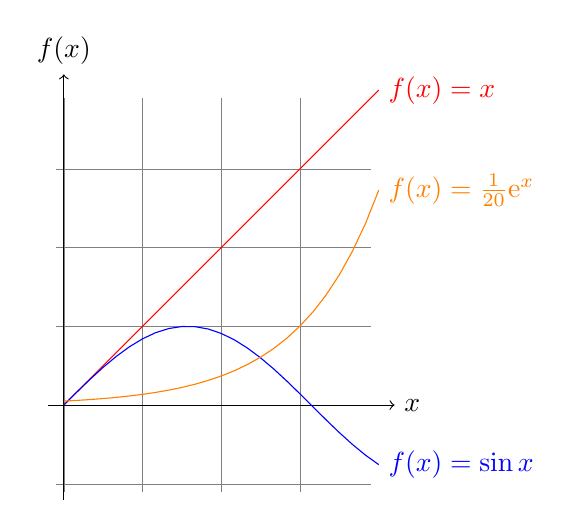
\begin{tikzpicture}[domain=0:4]
		  \draw[very thin,color=gray] (-0.1,-1.1) grid (3.9,3.9);
  		\draw[->] (-0.2,0) -- (4.2,0) node[right] {$x$};
		  \draw[->] (0,-1.2) -- (0,4.2) node[above] {$f(x)$};
		  \draw[color=red]    plot (\x,\x)             node[right] {$f(x) =x$};
  % \x r 表示弧度
		  \draw[color=blue]   plot (\x,{sin(\x r)})    node[right] {$f(x) = \sin x$};
		  \draw[color=orange] plot (\x,{0.05*exp(\x)}) node[right] {$f(x) = \frac{1}{20} \mathrm e^x$};
		\end{tikzpicture}
	\end{center}
\end{minipage}


\clearpage

\begin{minipage}<t>[htpb][80mm][t]{80mm}
	\begin{center}
		\vspace*{60mm}
    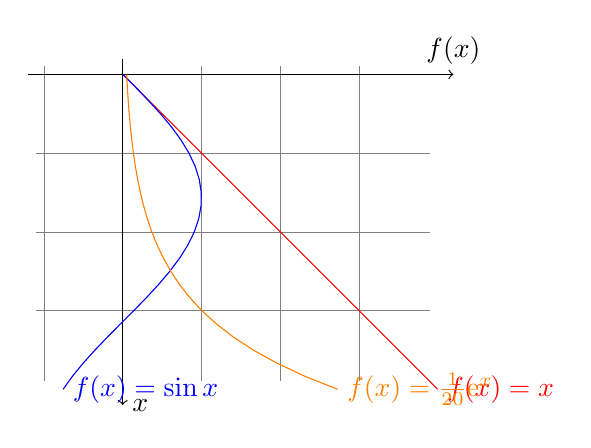
\begin{tikzpicture}[domain=0:4,scale=1,rotate=270]
		  \draw[very thin,color=gray] (-0.1,-1.1) grid (3.9,3.9);
  		\draw[->] (-0.2,0) -- (4.2,0) node[right] {$x$};
		  \draw[->] (0,-1.2) -- (0,4.2) node[above] {$f(x)$};
		  \draw[color=red]    plot (\x,\x)             node[right] {$f(x) =x$};
  % \x r 表示弧度
		  \draw[color=blue]   plot (\x,{sin(\x r)})    node[right] {$f(x) = \sin x$};
		  \draw[color=orange] plot (\x,{0.05*exp(\x)}) node[right] {$f(x) = \frac{1}{20} \mathrm e^x$};
		\end{tikzpicture}
	\end{center}
\end{minipage}

\chapter{公式測試}

\begin{minipage}<y>[htpb]{100mm}
		\vspace*{50mm}
	%\begin{center}
			{\normalsize With normalsize 10 pt in class (truely 10\,pt in real dimen):
				\[ \sampleEq \]\par}

			{\Large With Large 12 pt in class (truely 12\,pt in real dimen):
				\[ \sampleEq \]\par}

			{\footnotesize With footnotesize 8 pt in class (truely 8\,pt in real dimen):
				\[ \sampleEq \]\par}
	%\end{center}
\end{minipage}

\clearpage
\begin{minipage}<t>[htpb]{120mm}
		\vspace*{10mm}
	%\begin{center}
			{\normalsize 
				\[ \sampleEq \]\par}

			{\Large 
				\[ \sampleEq \]\par}

			{\footnotesize
				\[ \sampleEq \]\par}
	%\end{center}
\end{minipage}


\endinput

% 正文9pt 選擇 szix 選項
%\input{TESTTEXT/testtext9}

% 正文10pt 選擇 szx 選項
\input{TESTTEXT/testtext10}


% 正文11pt 選擇 szxi 選項
%% As a sample.tex gernerate by uplatex				%請使用uplatex編譯
% uplatex mysample && ptex2pdf -l -u -ot "-kanji=utf8 " -od "-p B5"  mysample

\szlarge
\chapter{測試}

\par\noindent
\ztxt{1A1}{\color{cyan}%
\kansuji12345\kansuji67890
\kansuji12345\kansuji67890
\kansuji12345\kansuji67890
\kansuji12345\kansuji67890
\kansuji12345\kansuji67890\\
頭注字號{9.13}\rensuji{pt}\\\rensuji{@}11.869\rensuji{pt},
行十字。}
\kansuji12345\kansuji67890
\kansuji12345\kansuji67890
\kansuji12345\kansuji67890
\kansuji12345\kansuji67890
\hspace{1zw}使用\verb+\szlarge+命令調用\dash\\
正文字號\rensuji{17}\rensuji{pt}\rensuji{@}\rensuji{30}\rensuji{pt},
一行\rensuji{28}至\rensuji{29}字不等。正文與割注換算關係為:

\begin{center}
一個正文字 = 1.90 割注字\footnote{脚注測試:序號為一}
\\%
\setcounter{footnote}{98}
一個正文字 = 2 行間注字\footnote{脚注測試:序號最大為九十九}
\endnote{需使用以下命令為行間注設置字號,使之恰好為正文字號的一半。\\  \hspace{2zw}
{\ttfamily $\backslash$rubyfontsetup\{$\backslash$mgfamily
$\backslash$fontsize\{9.31pt\}\{10\}$\backslash$selectfont\} }\\[2mm]
另一個方法,自動模式:不設置字號,只設置字體風格,默認振假名為正文字號的一半。如:\\ \hspace{2zw}
{\ttfamily $\backslash$rubyfontsetup\{$\backslash$mgfamily$\backslash$selectfont\} }}
\end{center}

\clearpage
\par\noindent\warichu*{%
\kansuji12345\kansuji67890
\kansuji12345\kansuji67890
\kansuji12345\kansuji67890
\kansuji12345\kansuji67890
\kansuji12345\kansuji67890
\kansuji12345\kansuji67
&%
\kansuji12345\kansuji67890
\kansuji12345\kansuji67890
\kansuji12345\kansuji67890
\kansuji12345\kansuji67890
\kansuji12345\kansuji67890
\kansuji12345\\
雙行割注字號{9.13}pt\rensuji{@}{9.13}pt in real diemen,&行\rensuji{55}字。}



\par\noindent{\normalsize
正文 normalsize,字號\rensuji{10}\rensuji{pt}\rensuji{@}\rensuji{18}\rensuji{pt},
行\rensuji{45}字。\\
\kansuji12345\kansuji67890
\kansuji12345\kansuji67890
\kansuji12345\kansuji67890
\kansuji12345\kansuji67890
\kansuji12345\kansuji67890
\kansuji12345\kansuji67890}


\par\noindent{\fontsize{11pt}{12}\selectfont
測試字號{10.043}\rensuji{pt}\rensuji{@}{10.043}\rensuji{pt},
行\rensuji{50}字。\\
\kansuji12345\kansuji67890
\kansuji12345\kansuji67890
\kansuji12345\kansuji67890
\kansuji12345\kansuji67890
\kansuji12345\kansuji67890
\kansuji12345\kansuji67890}

\clearpage
\theendnotes

\setcounter{chapter}{15}
\chapter{賈元春才選鳳藻宮 秦鯨卿夭逝黃泉路}

\par{}賈璉此時没好意思,
\ztxt{16A7}{\甲{〈庚〉:大觀園用省親事出題,是大関鍵事,方見大手筆行文之立意。\\\hfill{}畸笏。}}
只是訕笑吃酒,說「胡說」二字,「快盛飯来,吃碗子還要往珍大爺那邊去商議事呢。」鳳姐道:「可是別悞了正事。纔剛老爺叫你作什麼?」
\己{\warichu*{一段趙嫗討情閒文,却引出通部脈絡。所謂由小及大,譬如登高必自卑之意。細&思大觀園一事,若從如何奉旨起造,又如何分派衆人,從頭細細直冩將来,幾千\\{}樣細事,如何能順筆一氣冩清?又將落於死板拮据之鄕,故只用璉鳳夫妻二人一問一答,上用&趙嫗討情作引,下用蓉薔来說事作收,餘者隨筆順筆略一點染,則耀然洞徹矣。此是避難法。}}
賈璉道:「就爲
\ruby[Sg]{{\kenten{省親}。」鳳姐忙問}}{{\甲{二字醒眼之極,却只如此冩来。}}}
道:\甲{\warichu*{「忙」字最要緊,特於鳳姐口中出此字,可&知事関巨要,非同淺細,是此書中正眼矣。}}
「省親的事竟準了不成?」\甲{\warichu*{問得珍重,可知是萬&人意外之事。(脂硯)}}
賈璉笑道:「雖不十分準,也有八分準了。」
\甲{\warichu*{如此故頓一筆更妙!&見得事関重大,非一\\{}語可了者,亦是大篇&文章,抑揚頓挫之至。}}
鳳姐笑道:「可見當今的隆恩。歷来聽書看戲,古時從未有的。」%
\甲{\warichu*{於閨閣中作此語,直與&〈擊壤〉同聲。(脂硯)}}
\ztxt{16A8}{\甲{趙媽一問是文章家進一步門庭法則。\\[3mm]〈庚〉:自政老生日,用降旨截住,賈母等進朝如此熱鬧,用秦業死岔開,只冩幾個「如何」,將潑天喜事交代完了,緊接黛玉回,璉、鳳閒話,以老嫗勾出省親事来。其千頭萬緒,合榫貫連,無一毫痕跡,如此等,是書多多,不能枚舉。想兄在青峺峰上,經煅煉後,參透重関至恒河沙數。如否,余曰萬不能有此機括,有此筆力,恨不得面問果否。嘆嘆!\\\hfill{}丁亥春。畸笏叟。}}
趙媽\odora{}又接口道:\zmark{16A8}「可是呢,我也老糊塗了。我聽見上\odora{}下\odora{}吵嚷了這些日子,什麼省親不省親,我也不理論他去;如今又說省親,到底是怎麼個原故?」
賈璉道:\ruby[g]{{「如今當今貼體}}{{\甲{大觀園一篇大文,千頭萬緒,}}}\\
\ruby[g]{{「萬人之心,世上至大莫如『孝』字,想来父母児女之性,皆是一理,}}{{\甲{從何處冩起,今故用賈璉夫妻問答之間,閒閒敘出,觀者已省大半。後再用蓉、薔二人重一渲染。便省却多少贅瘤筆墨。此是避難法。}}}\\
不是貴賤上分別的。當今自爲日夜侍奉太上皇、皇太后,尚不能略盡孝意,因見宮裡嬪妃才人等皆是入宮多年,以致抛離父母音容,豈有不思想之理?在児女思想父母,是分所應當。想父母在家,若只管思念児女,竟不能一見,倘因此成疾致病,甚至死亡,皆由朕躬禁錮,不能使其遂天倫之願,亦大傷天和之事。故啓奏太上皇、皇太后,每月逢二六日期,準其椒房眷屬入宮請安看視。于是太上皇、皇太后大喜,深讚當今至孝純仁,體天格物。因此二位老聖人又下旨意,說椒房眷屬入宮,未免有國體儀制,母女尚不能愜懷。竟大開方便之恩,特降諭諸椒房貴戚,除二六日入宮之恩外,凡有重宇別院之家,可以駐蹕関防之處,不妨啓請內廷鑾輿入其私第,庶可略盡骨肉私情、天倫中之至性。此旨一下,誰不踴躍感戴?現今周貴人父親已在家裡動了工了,修蓋省親別院呢。又有吳貴妃的父親吳天佑家,也往城外\ruby[g]{{踏看地方}}{{\甲{又一樣佈置。}}}去了。這豈非有八九分了?」




\chapter{畫圖測試}


\begin{minipage}<y>[htpb]{80mm}
	\begin{center}
    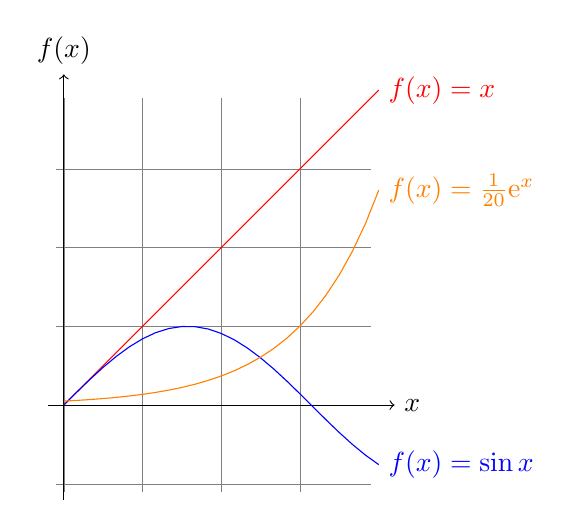
\begin{tikzpicture}[domain=0:4]
		  \draw[very thin,color=gray] (-0.1,-1.1) grid (3.9,3.9);
  		\draw[->] (-0.2,0) -- (4.2,0) node[right] {$x$};
		  \draw[->] (0,-1.2) -- (0,4.2) node[above] {$f(x)$};
		  \draw[color=red]    plot (\x,\x)             node[right] {$f(x) =x$};
  % \x r 表示弧度
		  \draw[color=blue]   plot (\x,{sin(\x r)})    node[right] {$f(x) = \sin x$};
		  \draw[color=orange] plot (\x,{0.05*exp(\x)}) node[right] {$f(x) = \frac{1}{20} \mathrm e^x$};
		\end{tikzpicture}
	\end{center}
\end{minipage}


\clearpage

\begin{minipage}<t>[htpb][80mm][t]{80mm}
	\begin{center}
		\vspace*{60mm}
    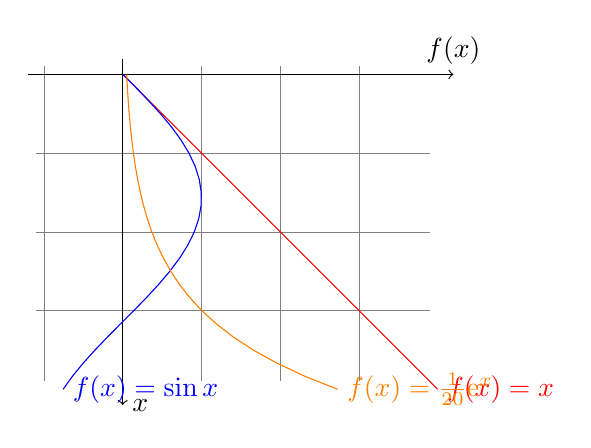
\begin{tikzpicture}[domain=0:4,scale=1,rotate=270]
		  \draw[very thin,color=gray] (-0.1,-1.1) grid (3.9,3.9);
  		\draw[->] (-0.2,0) -- (4.2,0) node[right] {$x$};
		  \draw[->] (0,-1.2) -- (0,4.2) node[above] {$f(x)$};
		  \draw[color=red]    plot (\x,\x)             node[right] {$f(x) =x$};
  % \x r 表示弧度
		  \draw[color=blue]   plot (\x,{sin(\x r)})    node[right] {$f(x) = \sin x$};
		  \draw[color=orange] plot (\x,{0.05*exp(\x)}) node[right] {$f(x) = \frac{1}{20} \mathrm e^x$};
		\end{tikzpicture}
	\end{center}
\end{minipage}

\chapter{公式測試}

\begin{minipage}<y>[htpb]{80mm}
		\vspace*{55mm}
	%\begin{center}
			{\normalsize With normalsize 10 pt in real dimen:
				\[ \sampleEq \]\par}

			{\Large With Large 14 pt in real dimen:
				\[ \sampleEq \]\par}

			{\footnotesize With footnotesize 8 pt in real dimen:
				\[ \sampleEq \]\par}
	%\end{center}
\end{minipage}

\clearpage
\begin{minipage}<t>[htpb]{120mm}
		\vspace*{10mm}
	%\begin{center}
			{\normalsize With normalsize 10 pt in real dimen:
				\[ \sampleEq \]\par}

			{\Large With Large 14 pt in real dimen:
				\[ \sampleEq \]\par}

			{\footnotesize With footnotesize 8 pt in real dimen:
				\[ \sampleEq \]\par}
	%\end{center}
\end{minipage}



\endinput


% 正文12pt 選擇 szxii 選項
%\input{TESTTEXT/testtext12}


% 正文 五號字(10.5pt) 選擇 xz 選項
%\input{TESTTEXT/testtext10x}


%%%%%% 自定義的封底
\cleardoublepage

\null\thispagestyle{empty}

\clearpage
\pagestyle{empty}
\ClearShipoutPictureBG
% 外封底

\begin{minipage}<y>[htpb]{.99\textheight}
\begin{center}
\vspace*{80mm} %奥付のページ上部からの位置
%\setlength\tabcolsep{3pt} %% 这个就是重点!!
\fontsize{9}{15}\selectfont\mgfamily\mdseries
	\begin{tabular}{cc}
		\multicolumn{2}{c}{\color{black}\huge\mcfamily\bfseries%
		\makebox[10zw][s]{脂硯齋重評石頭記}}
			\\[0pt] %%タイトル
		\multicolumn{2}{c}{\color{black}\rule{.99\textheight}{1pt}}
			\\[8pt]
		\hspace{5mm}\makebox[5zw][s]{\color{black}著 者}	&	%
		\makebox[36zw][l]{\color{black}\hspace{-.5zw}〔清〕曹雪芹}\\[0mm]  %%著者
		\hspace{5mm}\makebox[5zw][s]{\color{black}校者}	&	%
		\makebox[36zw][l]{\color{black}逍遙公子(三校)、雷明(四校)}\\[0mm]  %%校訂
		\hspace{5mm}\makebox[5zw][s]{\color{black}紙 張}	&	%
		\makebox[36zw][l]{\color{black}JIS B5(182×257mm)}\\[0mm]  %%尺寸
		\hspace{5mm}\makebox[5zw][s]{\color{black}行 款}	&	%
		\makebox[36zw][l]{\color{black}每頁十四行;每行卅五字}\\[0mm]  %%尺寸
		\hspace{5mm}\makebox[5zw][s]{\color{black}發 行 人}	&	%
		\makebox[36zw][l]{\color{black}子 康(Steve Cheung)}\\[0mm]  %%發行人
		\hspace{5mm}\makebox[5zw][s]{\color{black}聯 繫 方 式}	&	%
		\makebox[36zw][l]{\color{black} 602644360@qq.com}\\[0mm]  %%發行者
		\hspace{5mm}\makebox[5zw][s]{\color{black}當 前 版 本}	&	%
		\makebox[36zw][l]{\color{black} v2.006-20240312}\\[0mm]  %%版本
		\hspace{5mm}\makebox[5zw][s]{\color{black}發 行 日}	&	%
		\makebox[36zw][l]{\color{black}{\number\year}~年~{\number\month}~月~{\number\day}~日 }%%發行日
			\\[0pt] 
		\multicolumn{2}{c}{\color{black}\rule{.99\textheight}{1pt}}
			\\[3pt]
		\multicolumn{2}{c}{\color{black}本書電子版僅提供屏幕試閱。請勿印刷傳播。 對於書中錯漏,鄙人不擔負任何責任及義務。}%%免責申明
			\\[0mm]
		\multicolumn{2}{c}{\color{black}本書不刻意追求完美,允許少量錯別字存在。 若是發現排版錯誤,敬請截圖發到我的信箱。}%%免責申明
			\\[0pt] 
		\multicolumn{2}{c}{\color{black}\rule{.99\textheight}{1pt}}
			\\[3pt]
		\multicolumn{2}{r}{\color{black}{\mgfamily\mdseries%
			\hbox{}\hfill\CID{734}商用禁止;轉載自由(保留署名)}} 
	\end{tabular}
\end{center}
\end{minipage}


\endinput




\end{document}